\documentclass[tikz,border=5pt]{standalone}
\usepackage{amsmath,amssymb}
\begin{document}
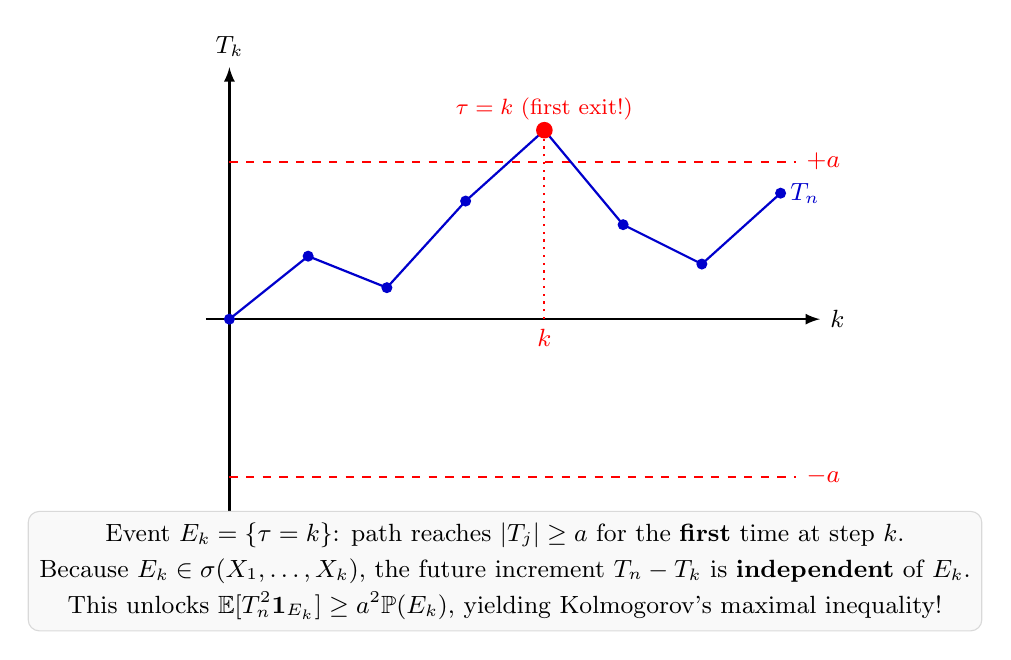
\begin{tikzpicture}[>=latex, font=\small]
  % Axes
  \draw[->, thick] (0, -2.5) -- (0, 3.2) node[above] {$T_k$};
  \draw[->, thick] (-0.3, 0) -- (7.5, 0) node[right] {$k$};

  % Threshold lines
  \draw[dashed, red, thick] (0, 2.0) -- (7.2, 2.0) node[right] {$+a$};
  \draw[dashed, red, thick] (0, -2.0) -- (7.2, -2.0) node[right] {$-a$};

  % Path
  \draw[thick, blue!80!black] (0, 0)
    -- (1, 0.8)
    -- (2, 0.4)
    -- (3, 1.5)
    -- (4, 2.4) node[above, font=\footnotesize, red] {$\tau = k$ (first exit!)}
    -- (5, 1.2)
    -- (6, 0.7)
    -- (7, 1.6);

  \fill[blue!80!black] (0, 0) circle (2pt);
  \fill[blue!80!black] (1, 0.8) circle (2pt);
  \fill[blue!80!black] (2, 0.4) circle (2pt);
  \fill[blue!80!black] (3, 1.5) circle (2pt);
  \fill[red] (4, 2.4) circle (3pt);
  \fill[blue!80!black] (5, 1.2) circle (2pt);
  \fill[blue!80!black] (6, 0.7) circle (2pt);
  \fill[blue!80!black] (7, 1.6) circle (2pt) node[right] {$T_n$};

  \draw[dotted, red, thick] (4, 0) -- (4, 2.4);
  \node[below, red] at (4, 0) {$k$};

  \node[align=center, fill=gray!5, draw=gray!30, rounded corners, inner sep=4pt] at (3.5, -3.2)
    {Event $E_k = \{\tau = k\}$: path reaches $|T_j| \ge a$ for the \textbf{first} time at step $k$.\\[2pt]
     Because $E_k \in \sigma(X_1, \dots, X_k)$, the future increment $T_n - T_k$ is \textbf{independent} of $E_k$.\\[2pt]
     This unlocks $\mathbb{E}[T_n^2 \mathbf{1}_{E_k}] \ge a^2 \mathbb{P}(E_k)$, yielding Kolmogorov's maximal inequality!};
\end{tikzpicture}
\end{document}
